\chapter{Results}
\label{chp:results}

In this chapter the results of the project will be shown. This contains measurements of transmission of 4 images. No compression, 1-bit compression, 2-bit compression and 4-bit compression.

To get the results, an image was send between two TelosBs, one as a sender and one as a receiver. These was implemented as described in chapter \ref{chp:impl}

Three different compressions was developed, and each with a different result, as expected. As shown i figure \ref{fig:one}, \ref{fig:two} and \ref{fig:four}.

\todo{indsæt rette billeder}
\begin{figure}[h]
	\centering
	\begin{subfigure}{0.3\textwidth}
		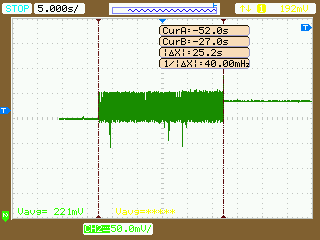
\includegraphics[width=\textwidth]{senderResultconverted}
		\caption{1-bit compression}
		\label{fig:one}
	\end{subfigure}
	\begin{subfigure}{0.3\textwidth}
		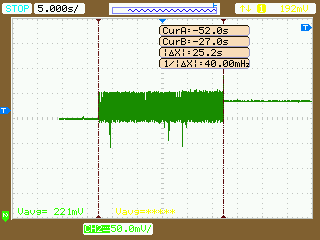
\includegraphics[width=\textwidth]{senderResultconverted}
		\caption{2-bit compression}
		\label{fig:two}
	\end{subfigure}
	\begin{subfigure}{0.3\textwidth}
		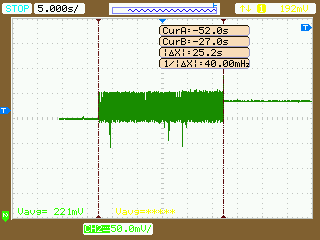
\includegraphics[width=\textwidth]{senderResultconverted}
		\caption{4-bit compression}
		\label{fig:four}
	\end{subfigure}
	\caption{Pictures of animals}\label{fig:animals}
\end{figure}


To measure the voltage over the mote and the transmission time, a oscilloscope was used. Figure \ref{fig:senderresult} shows the measurement of no compression from the sender. 

\myFigure{senderResultconverted}{Mesured values for no compressed on sender side}{fig:senderresult}{0.6}


The table below shows all measurements and calculations of the 3 compressions and one transmission without any compression.

\begin{tabular}{l l l l r r r r r}
	Sender           	& $V_{avg}\lbrack mV\rbrack$ & $Res\lbrack \Omega\rbrack$ & $V_{bat}\lbrack V\rbrack$ & $t\lbrack sec\rbrack$ & $V_{mote}$  & $I_{mote}$ & $W_{mote}\lbrack W\rbrack$ & Energy cons.\\ \hline
	No compr.	 & 0.194 & 9.93 & 3.028 & 25.2 & 2.834 & 0.020 & 0.055 & 1.395 \\
	1-bit compr. & 0.192 & 9.93 & 3.028 & 24.5 & 2.836 & 0.019 & 0.055 & 1.343 \\
	2-bit compr. & 0.193 & 9.93 & 3.028 & 23   & 2.835 & 0.019 & 0.055 & 1.267 \\
	4-bit compr. & 0.194 & 9.93 & 3.028 & 18.2 & 2.834 & 0.020 & 0.055 & 1.008 \\
	
	&&&&&&&& \\

	Receiver           	& $V_{avg}\lbrack mV\rbrack$ & $Res\lbrack \Omega\rbrack$ & $V_{bat}\lbrack V\rbrack$ & $t\lbrack sec\rbrack$ & $V_{mote}$  & $I_{mote}$ & $W_{mote}\lbrack W\rbrack$ & Energy cons.\\ \hline
	No compr.	 & 0.201 & 9.98 & 3.214 & 25.2 & 3.013 & 0.020 & 0.060 & 1.529 \\
	1-bit compr. & 0.201 & 9.98 & 3.214 & 24.5 & 3.013 & 0.020 & 0.060 & 1.487 \\
	2-bit compr. & 0.2   & 9.98 & 3.214 & 23   & 3.014 & 0.020 & 0.060 & 1.389 \\
	4-bit compr. & 0.2   & 9.98 & 3.214 & 18.2 & 3.014 & 0.020 & 0.060 & 1.099
\end{tabular}

Before transmission of images the resistanse of the resistor and voltage of the battery was measured. This is done to calculate $V_{mote}$, $I_{mote}$, $W_{mote}$ and \emph{energy consumption}. Below the calculations are shown:
 
\begin{align*}
	V_{bat}&=V_{bat}-V_{res}\\
	I_{mote}&= \dfrac{V_{avg}}{Res}\\
	W_{mote}&=I_{mote}\cdot V_{mote} \\
	EC&=W_{mote}\cdot t
\end{align*}